\chapter{Analisi dei muoni cosmici in JUNO}
\label{cap:muon}
Lo studio dei muoni che interagiscono all'interno di JUNO è di fondamentale importanza per la maggior parte delle misure scientifiche di interesse. Questo lavoro di tesi si concentra sull’analisi dei primi dati provenienti da JUNO durante la fase di riempimento con lo scintillatore liquido. I dati analizzati partono da gennaio 2025 e finiscono a marzo 2025.

Caratterizzare con precisione la traccia dei muoni all’interno del rivelatore è il primo passo per sviluppare la tecnica di veto, utile a ridurre il background da isotopi cosmogenici descritto nel capitolo precedente. A tal fine, sono stati utilizzati due metodi per l'identificazione dei muoni. Il primo metodo, sfrutta la correlazione temporale tra gli eventi registrati nel CD e nella WP, mentre il secondo analizza la formazione di gruppi (cluster) di PMT attivati nella WP. Entrambi gli approcci si basano sulla notevole energia dei muoni, che attivano con altissima  probabilità la finestra di trigger per l'acquisizione degli eventi. Questi due metodi costituiscono solo una parte della strategia complessiva per la classificazione e caratterizzazione degli eventi candidati muoni. In questo capitolo verranno illustrati il loro funzionamento, i risultati ottenuti e un confronto tra le due metodologie.
\section{La tecnica di veto per i muoni cosmici}
I muoni cosmici, come accennato nella sezione \ref{sec:fondi}, rappresentano la principale sorgente di background cosmogenico nel rivelatore centrale di JUNO. Situato sotto uno strato di roccia di $700\,\unit{m}$, JUNO risulta comunque esposto a un flusso residuo di muoni pari a $\sim 4\,\unit{mHz/m^2}$.

Le simulazioni Monte Carlo stimano un rate di muoni pari a $\sim4\,\unit{Hz}$ nel CD e $\sim10.5\,\unit{Hz}$ nella WP. Con un'energia media di circa $209\,\unit{GeV}$, queste particelle elementari relativistiche possono indurre la produzione di isotopi radioattivi o neutroni liberi all'interno del CD, contribuendo così al background sperimentale. Poiché l'energia media dei muoni cosmici è così elevata, il loro passaggio attraverso il rivelatore è accompagnato da una forte emissione di luce Cherenkov. Sfruttando la relazione di Frank-Tamm:

\begin{equation} 
    \frac{dN_\gamma}{dxd\lambda}=\frac{2\pi\alpha z^2}{\lambda^2}\sin^2{\theta_c(\lambda)} 
\end{equation}
dove $z$ è la carica della particella, $\alpha$ è la costante di struttura fine, $\lambda$ è la lunghezza d'onda e $\theta_c$ è l'angolo caratteristico del cono Cherenkov. Questa espressione può essere semplificata inserendo i valori tipici di $\lambda$ per l'emissione Cherenkov, che si collocano nella regione del vicino ultravioletto. Inoltre, assumendo che il muone sia una particella relativistica con carica $z=1$, si ottiene che il numero di fotoni Cherenkov prodotti è approssimativamente $N_\lambda \approx 5 \cdot 10^{4}\,\unit{m^{-1}}$. La quantità di fotoelettroni misurata dai PMT risulta inferiore a causa di diversi fattori, tra cui l'efficienza quantica \ref{eq:qe} e gli effetti di propagazione ottica. Nonostante queste attenuazioni, il segnale prodotto dal passaggio dei muoni è nettamente superiore rispetto a quello della radioattività, che si colloca tipicamente nell'ordine del MeV. Per il CD, in base a stime preliminari e simulazioni Monte Carlo, ad $1\,\unit{MeV}$ di energia depositata corrispondono circa $1500$ fotoelettroni prodotti dai PMT. Nel caso di muoni, qualitativamente ci si aspetta un'energia depositata almeno cento volte superiore rispetto al fondo radioattivo.

L'elevato numero di fotoni Cherenkov è in grado di attivare un numero significativo di PMT, innescando così l'apertura della finestra di trigger di acquisizione. Durante la fase di riempimento, la finestra di trigger $220\,\unit{ns}$ si attiva quando all'interno di questo intervallo di tempo vengono rivelati circa $200$ fotoelettroni. Una volta identificato un evento candidato muone, l'idea chiave per la riduzione del fondo di isotopi cosmogenici si basa sulla ricostruzione della traiettoria dei muoni attraverso il CD. Questa tecnica di veto consiste nel definire via software una regione di esclusione attorno alla traccia del muone, all'interno della quale gli eventi vengono scartati per un certo intervallo temporale. Una rappresentazione schematica di questa strategia è mostrata in Figura \ref{Fig:muon_vet}. Quello che viene fatto è selezionare una zona cilindrica attorno all'evento muone interno al CD in cui non vengono analizzati i dati poichè la probabilità che contenga isotopi cosmogenici è molto alta.
%Immagine provvisoria
\begin{figure}[h!]
\centering
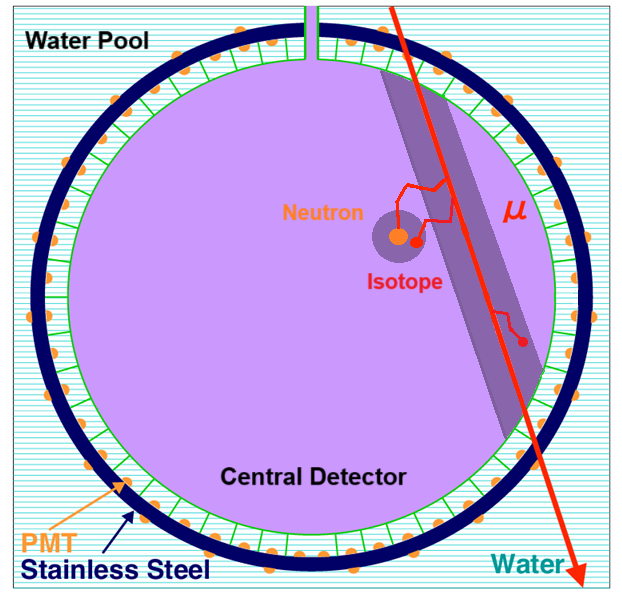
\includegraphics[width=0.4\textwidth]{Immagini/Ritentativo.png}
\caption{Schema del rivelatore centrale e la tecnica di veto per i muoni e i neutroni liberi.}
\label{Fig:muon_vet}
\end{figure}
La dimensione del raggio del cilindro di veto viene modulata in funzione della presenza di un muone singolo o di un bundle e a seconda dell'analisi di interesse. Nel caso di neutroni liberi, invece, viene definita una regione di veto di forma sferica attorno alla posizione ricostruita del neutrone interagente con LS.

L'obiettivo di questa tesi si colloca sul primo passo di questra strategia, cioè sulla classificazione degli eventi muone e sulla ricostruzione della traccia.
\section{La classificazione di un evento in JUNO}
I dati analizzati provengono direttamente dal rivelatore JUNO e sono suddivisi in \textit{Run}. Ogni \textit{Run} può essere costituita da diversi datasets ognuno associato al sotto-rivelatore preso in considerazione: il Central Detector (CD), la Water Pool (WP) o il Top Tracker (TT), installato nei primi giorni di marzo 2025 e non considerato nelle analisi discusse. 

Le \textit{Run} sono identificate univocamente con un codice numerico di quattro cifre (RUNXXXX).  Per ogni \textit{Run} analizzata sono stati generati tre file \texttt{.root}, contenenti tutte le informazioni estratte dalla presa dati ed elaborate dai diversi algoritmi di ricostruzione degli eventi. L'uso dei file ROOT consente una gestione più efficiente della grande mole di dati acquisiti. La Figura \ref{Fig:Diagramma} illustra la struttura dei dataset analizzati per le analisi di questa tesi:
\begin{itemize}
    \item \textbf{totalCD}: i file ROOT prodotti da questa elaborazioni contenente i TTrees "Events", che registrano l'intera popolazione di eventi nel Central Detector. Le informazioni di interesse per l'analisi sono: la carica in fotoelettroni prdotta dai PMT per ciascun evento e il tempo assoluto di trigger.
    \item \textbf{totalWP}: i file ROOT prodotti da questa elaborazione contengono TTrees "Events" in cui sono presenti la totalità degli eventi registrati nella Water Pool. Le informazioni analizzate sono le medesime per i file prodotti da totalCD.
    \item \textbf{WpMuonClassifyRecTool}: parte del software ufficiale di JUNO, questo algoritmo si occupa di selezionare dai dati totali della Water Pool solo gli eventi candidati muoni basandosi sul clustering di carica dei PMT della WP. Il funzionamento di identificazione di WpMuonClassifyRecTool verrà descritto nella sezione \ref{sec:wpmuonclassify}. I file \texttt{.root} contengono un TTrees "MuonsEvents". Questa struttura include dati relativi alla posizione di entrata e di uscita dell'evento candidato muone in coordinate cartesiane, i tre versori della direzione di propagazione dell'evento, il tempo assoluto di trigger della WP e la variabile intera trackID, che indica la molteplicità della traccia in caso di muoni bundle. Inoltre è indicata anche la carica in fotoelettroni prodotta dai PMT della WP.
\end{itemize}
\begin{figure}[h!]
\centering
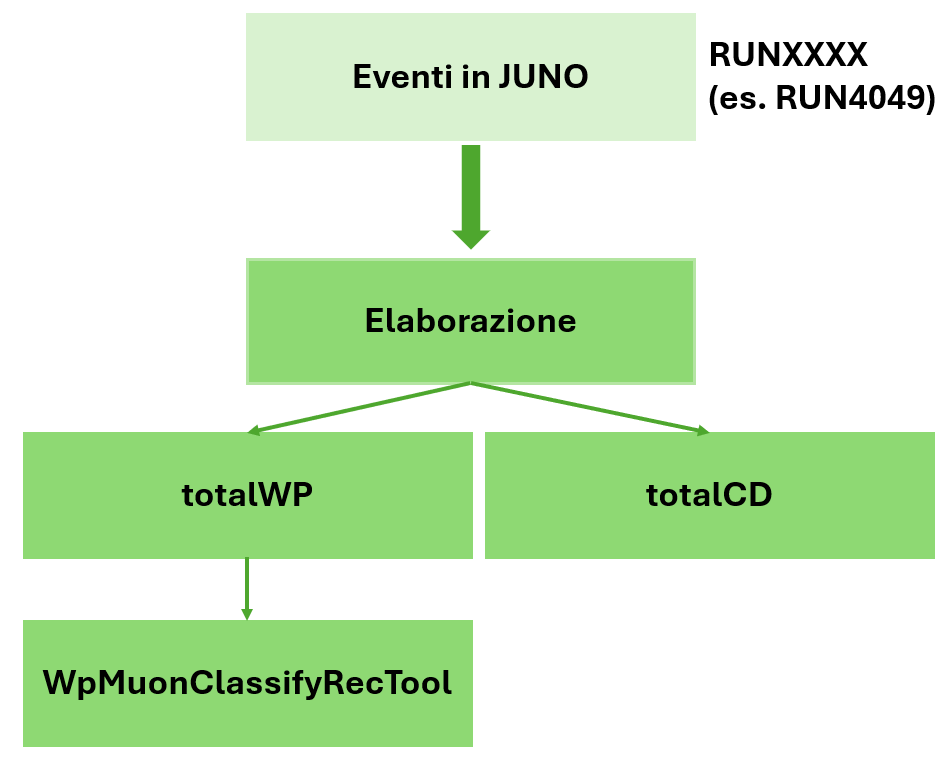
\includegraphics[width=0.6\textwidth]{Immagini/Diagramma.png}
\caption{Schema dei dataset analizzati per ogni \textit{Run}. I dataset \textbf{totalWP} e \textbf{totalCD} sono ottenuti ricostruendo tutti gli eventi eventi registrati rispettivamente nella WP e nel CD. \textbf{WpMuonClassifyRecTool} il quale è derivato da totalWP.}
\label{Fig:Diagramma}
\end{figure}
Tutti i dati contenuti nei TTrees sono accessibili attraverso la libreria CERN ROOT. L'analisi è stata condotta mediante un programma scritto in \texttt{C++}. A titolo di esempio, presento i risultati di una singola \textit{Run} rappresentativa: la RUN4049 è stata avviata alle 08:08 del 18 febbraio 2025, ha una durata complessiva di $14382.4\,\unit{s}$. I risultati completi sono stati raccolti e pubblicati all'interno di una repository su GitHub\footnote{Repository GitHub: \url{https://github.com/NicoFava/Tesi_V2.git}}, insieme all'intero codice sviluppato. 

Come discusso nella sezione precedente, l'energia media dei muoni cosmici è molto elevata e il loro passaggio attraverso il rivelatore è accompagnato da una forte emissione di luce Cherenkov. Quindi, la probabilità che un evento muone apra la finestra di trigger è molto alta. I PMT registrano la carica dell'evento in fotoelettroni, e lo spettro della carica totale raccolta nella Water Pool e nel Central Detector è riportato in Figura \ref{Fig:chargesample}.
 \begin{figure}[h!]
    \centering
    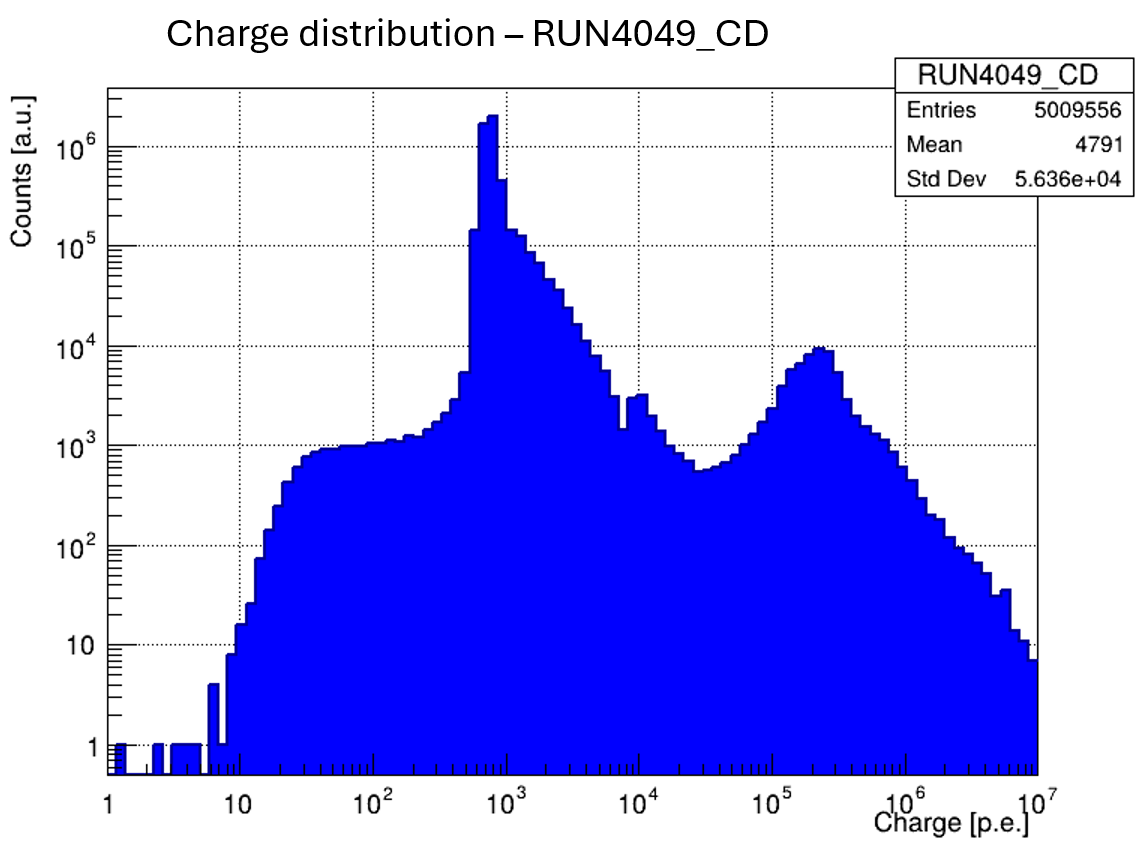
\includegraphics[width=0.49\textwidth]{Risultati/total_PeSum_log_RUN4049_CD.png}
    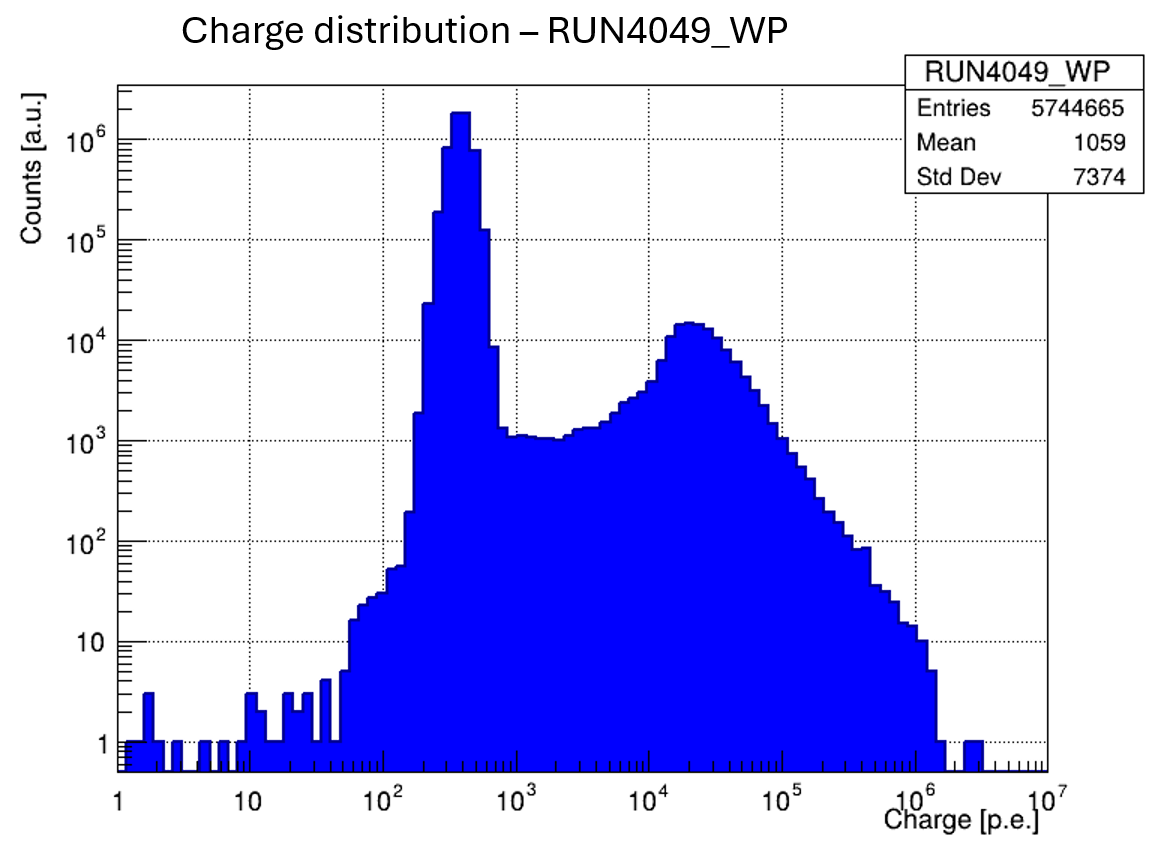
\includegraphics[width=0.5\textwidth]{Risultati/total_PeSum_log_RUN4049_WP.png}
    \caption{Spettro della carica in fotoelettroni degli eventi totali registrati nel Central Detector a sinistra e nella Water Pool a destra per la RUN4049.}
    \label{Fig:chargesample}
\end{figure}
\section{Metodo di correlazione temporale}
Usando come riferimento la Figura \ref{Fig:muon_vet}, un muone che attraversa prima la Water Pool e poi il Central Detector, essendo un evento ad alta energia, produce  l'apertura della finestra di trigger sia per i PMT della WP che per i PMT del CD ad un tempo assoluto diverso ma vicino. Approssimando i muoni come particelle relativistiche e considerando il diametro di $35\,\unit{m}$ del CD, il ritardo tra l'acquisizione dell'evento candidato muone nella WP ($t_\text{WP}$) e l'apertura della finestra di trigger nel CD ($t_\text{CD}$) dovrebbe essere nell'ordine di grandezza di $\Delta t\approx150\,\unit{ns}$. Questo valore qualitativo tiene anche conto del tempo necessario affinché i fotoni raggiungano i PMT e che questi diano un segnale.

Il metodo sviluppato si basa sulla correlazione temporale tra gli eventi registrati dai PMT della WP e del CD. Per identificare gli eventi correlati, ho implementato una funzione che accetta in input i due dataset totalCD e totalWP provenienti della stessa \textit{Run} e un valore di tolleranza temporale $t_\text{co}$. Variando il tempo di correlazione varia il numero di eventi comuni trovati con $\Delta t$ tale che:
\begin{equation}
    \Delta t = |t_{WP} - t_{CD}|\le t_\text{co}
    \label{eq:diff}
\end{equation}
Per ottimizzare questa metodologia, ho testato diversi valori per l'intervallo di tolleranza, variando da valori estremi di $1\,\unit{ns}$ fino a $1\,\unit{s}$, esplorando più ordini di grandezza per valutare al meglio il numero di eventi correlati in funzione del tempo di correlazione. Per ogni valore di tolleranza scelto (incrementato per fattori di 10), ho analizzato e confrontato lo spettro della carica degli eventi correlati con lo spettro della totalità degli eventi registrati. Questo ha permesso di ottenere una visione più chiara delle caratteristiche degli eventi candidati come muoni.

Un aumento della tolleranza temporale comporta un incremento degli eventi di fondo accidentalmente correlati a più bassa carica raccolta. Quindi, attraverso una scelta basata sull'osservazione degli spettri di carica è stato fissato un intervallo di tolleranza ($t_\text{co}$) e  applicato una selezione in carica sullo spettro della WP e del CD ($E^\text{WP}_\text{th}$ e $E^\text{CD}_\text{th}$). Una volta individuato un valore ottimale per la tolleranza temporale e un criterio di selezione basato sugli spettri di carica, ho calcolato il rate di eventi muone per ogni \textit{Run} utilizzando questo metodo.
\subsection{Studio preliminare}
Il primo passo per candidare gli eventi muoni attraverso il metodo di correlazione temporale è determinare quanti eventi possono essere effettivamente correlati. Prendendo come esempio i due datasets totalCD e totalWP provenienti dalla RUN4049, ho analizzato il numero totale di eventi correlati al variare del tempo di correlazione $t_\text{co}$ su diversi ordini di grandezza, inclusi tempi estremi. L'istogramma in Figura \ref{Fig:corr1} mostra il numero totale di eventi correlati nei dataset totalWP e totalCD in funzione del tempo di correlazione $t_\text{co}$.

\begin{figure}[h!]
    \centering
    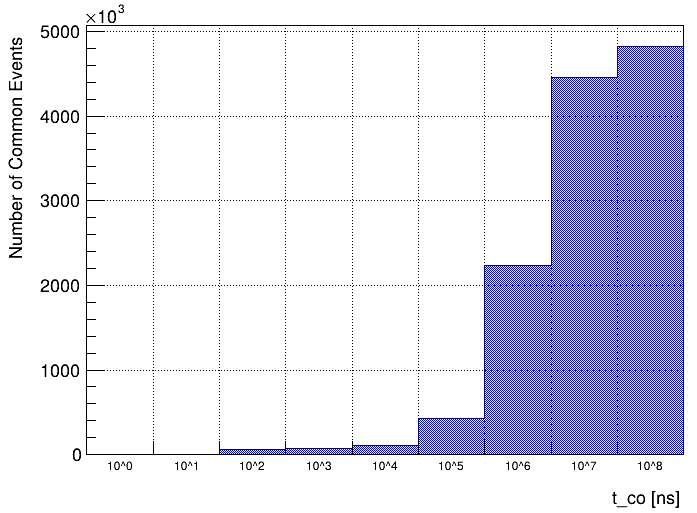
\includegraphics[width=0.6\textwidth]{Risultati/Common_Events_vs_Tolerance_RUN4049_plot.png}
    \caption{Distribuzione del numero di eventi correlati al variare di $t_\text{co}$ per la RUN4049.}
    \label{Fig:corr1}
\end{figure}
Come previsto, all'aumentare della finestra temporale, aumenta il numero di eventi correlati, ma con essi crescono anche gli eventi di fondo casualmente associati. Questo indica che questo metodo, basandosi solo sul tempo assoluto, introduce inevitabilmente un certo grado di rumore. Senza effettuare alcuna selezione in carica negli spettri della WP e del CD, il rate degli eventi correlati in funzione della finestra temporale è riportato in Figura \ref{Fig:corre2}, dove si nota come a un tempo di correlazione maggiore il rate degli eventi candidati risulta molto superiore rispetto ai valori ragionevolmente attesi, nell'ordine di grandezza degli $\unit{Hz}$.
\begin{figure}[h!]
    \centering
    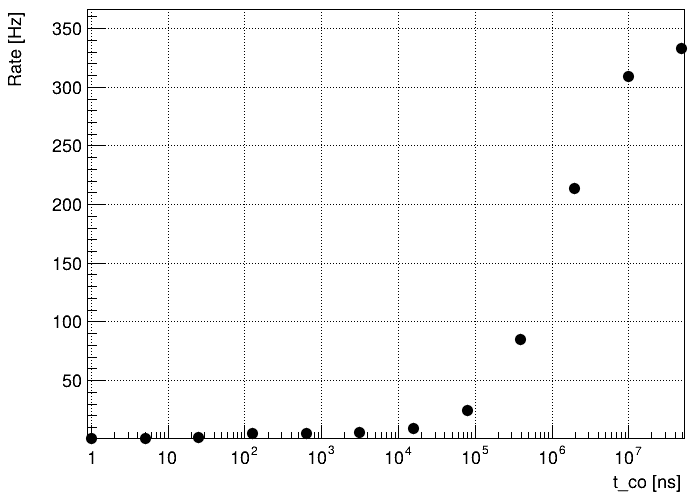
\includegraphics[width=0.6\textwidth]{Risultati/Common_Events_vs_Tolerance_RUN4049_rate_plot.png}
    \caption{Rate della RUN4049 degli eventi candidati muoni solo attraverso il tempo assoluto in funzione dei diversi intervalli di tempo di correlazione. Le barre di errore sono presenti ma non visibili poichè trascurabili rispetto ai valori di rate.}
    \label{Fig:corre2}
\end{figure}
\subsection{Selezione del tempo di correlazione e della soglia di carica}
\label{sec:aba}
Per affinare il metodo è stato necessario considerare gli spettri di carica degli eventi candidati per diversi valori del tempo di correlazione. La Figura \ref{Fig:common} mostra gli spettri di carica del CD (a sinistra) e della WP (a destra), fissando $t_\text{co}=200\,\unit{ns}$. Come evidenziato dalla Figura \ref{Fig:poker}, in cui è rappresentato lo spettro della carica nel CD variando il tempo di tolleranza, il numero di eventi a bassa carica aumenta all'aumentare del tempo di correlazione. Con alta probabilità, questi eventi sono principalmente dovuti a coincidenze accidentali di rumore dei PMT, ma potrebbero anche essere influenzati dai fondi radioattivi intrinseci dell'acqua e dello scintillatore. Basandomi su queste osservazioni, ho scelto empiricamente una soglia per lo spettro WP e lo spettro CD. Nell'appendice \ref{sec:appen} è possibile osservare la variazione dello spettro della carica in fotoelettroni per gli eventi rivelati nella Water Pool.
%cambiare titolo nomi ecc ecc
\begin{figure}[h!]
    \centering
    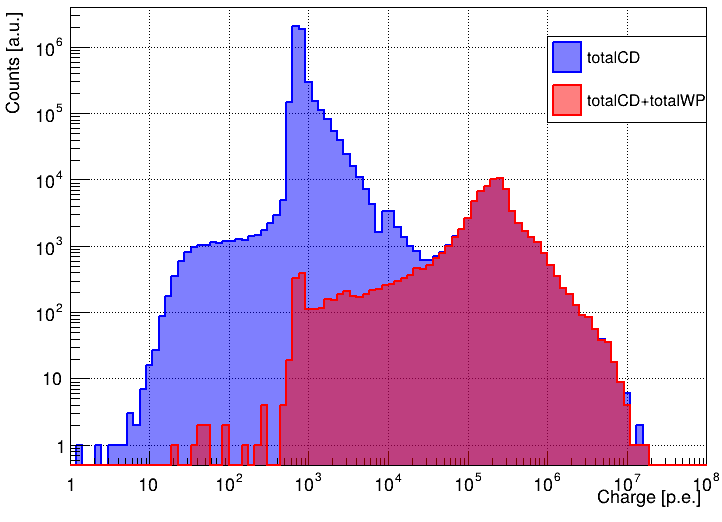
\includegraphics[width=0.49\textwidth]{Risultati/CD_RUN4049_tolerance_200.00.png}
    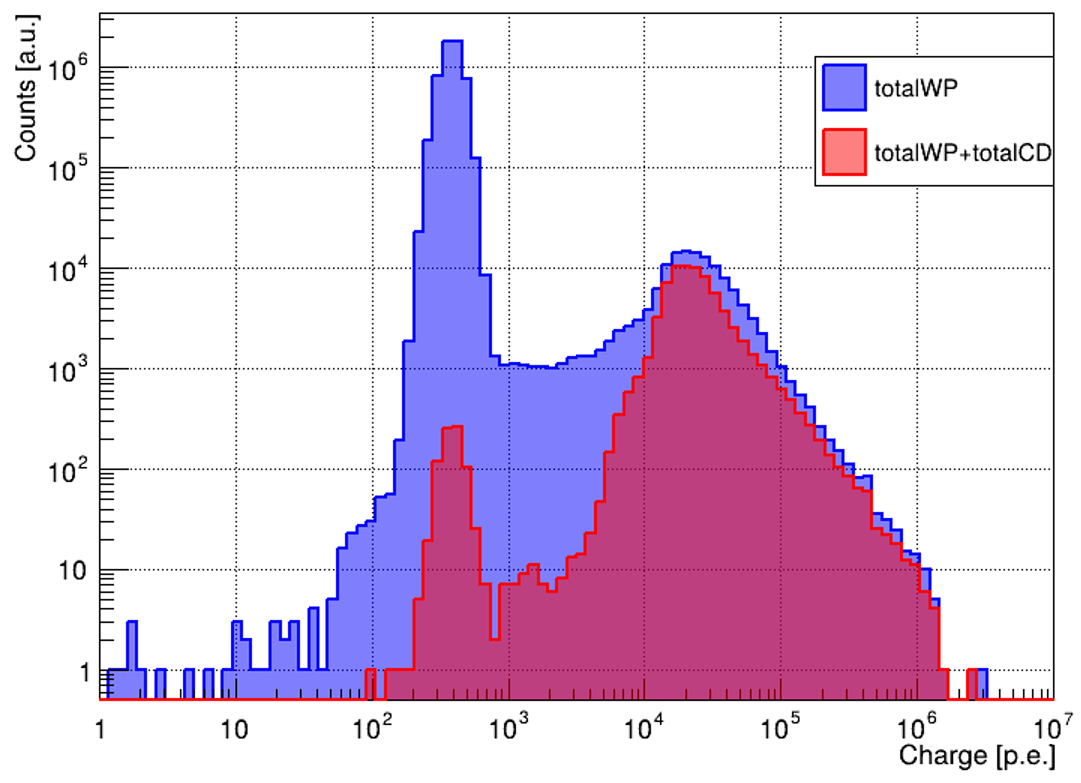
\includegraphics[width=0.49\textwidth]{Risultati/WP_RUN4049_tolerance_200.00.png}
    \caption{Spettri di carica raccolta nel CD (a sinistra) nella WP (a destra) per la RUN4049. In blu lo spettro della carica totale in rosso lo spettro degli eventi selezionati tramite correlazione temporale. }
    \label{Fig:common}
\end{figure}
Oltre alla soglia di carica è anche possibile osservare che la porzione di spettro superiore alla selezione effettuata risulta pressochè invariato mentre gli eventi a bassa carica tendono ad aumentare con l'aumentare del tempo di correlazione. Di conseguenza, i valori impostati sono i seguenti:
\begin{itemize}
    \item Tempo di correlazione: $t_\text{co}=200\,\unit{ns}$;
    \item Soglia nella WP: $E^\text{WP}_\text{th} = 5\cdot10^3\,\text{p.e.}$;
    \item  Soglia nel CD: $E^\text{CD}_\text{th} = 5\cdot10^4\,\text{p.e.}$.
\end{itemize}
\begin{figure}[h!]
\centering
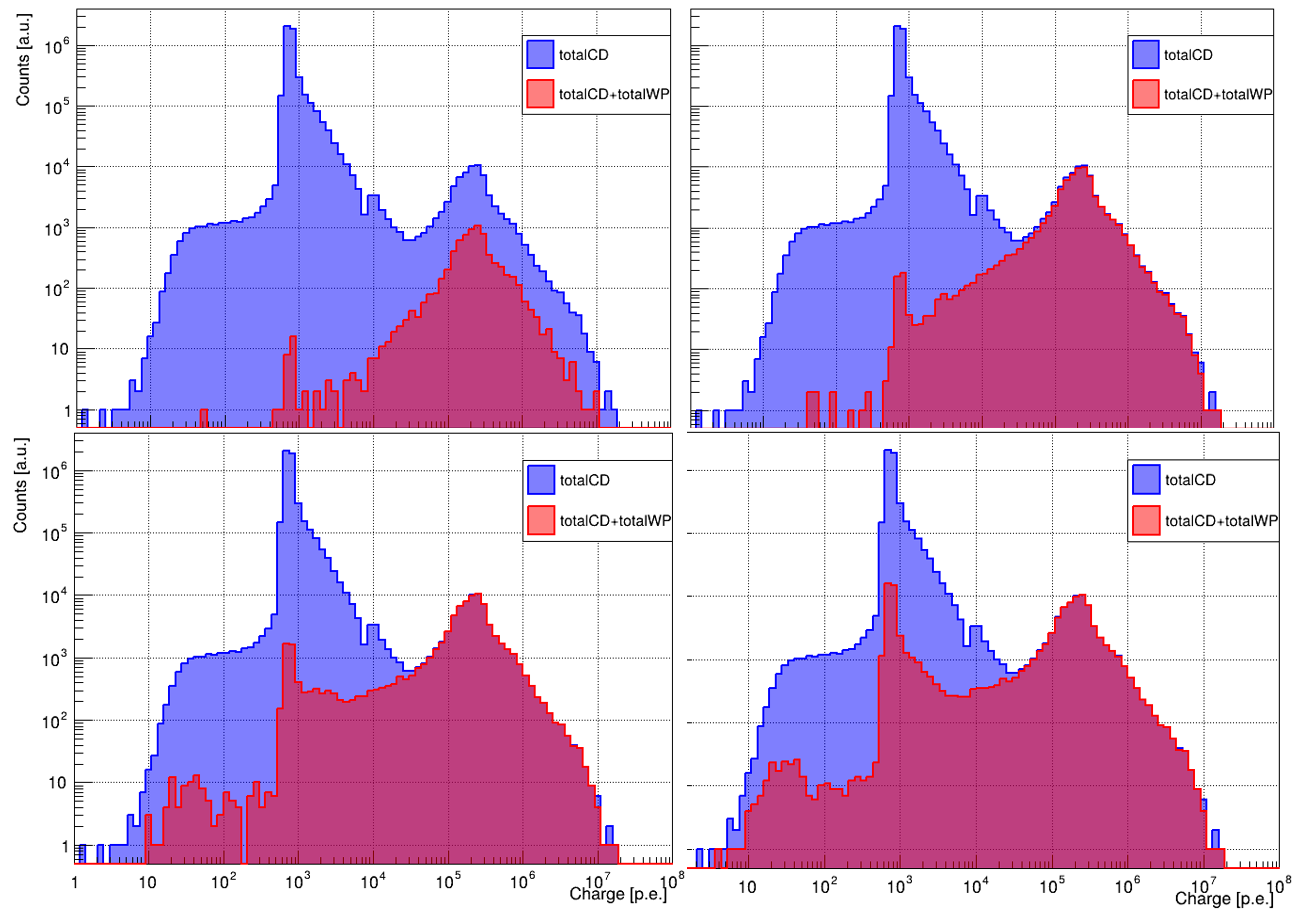
\includegraphics[width=0.75\textwidth]{Risultati/poker.png}
\caption{Spettro della carica in fotoelettroni del Central Detector per la RUN4049. Il tempo di correlazione è $10\,\unit{ns}$ per lo spettro in alto a sinistra, $100\,\unit{ns}$ in alto a destra, $1000\,\unit{ns}$ in basso a sinistra e $10000\,\unit{ns}$ in basso a destra.}
\label{Fig:poker}
\end{figure}
La scelta della soglia di carica nello spettro del Central Detector risulta più complessa rispetto a quella nella Water Pool. Infatti, mentre nello spettro della WP è possibile identificare un valore chiaro che separa gli eventi a bassa carica da quelli ad alta carica raccolta dai PMT della WP, nel caso del CD non esiste una soglia netta che permetta una distinzione altrettanto evidente. Dopo aver applicato queste soglie, il nuovo rate in funzione del tempo di correlazione è mostrato in Figura \ref{Fig:ratez}. A sinistra è riportato il grafico del rate in funzione del tempo di correlazione applicando la selezione in carica nello spettro WP, mentre a destra è mostrato lo stesso grafico applicando la selezione nello spettro CD. Fissando il tempo di correlazione e le selezioni in carica nei due spettri ai valori indicati precedentemente, si ottengono i seguenti valori per il rate degli eventi candidati muoni:
\begin{align}
\text{Selezione in carica WP:} \quad \text{rate}\,(\text{RUN}4049) = (4.04\pm0.02)\,\unit{Hz}\label{eq:rateWP}\\
\text{Selezione in carica CD:} \quad \text{rate}\,(\text{RUN}4049) = (4.62\pm0.02)\,\unit{Hz}
\label{eq:rateCD}
\end{align}
l'errore è stato calcolato assumendo che il numero di eventi segua la distribuzione di Poisson.
\begin{figure}[h!]
\centering
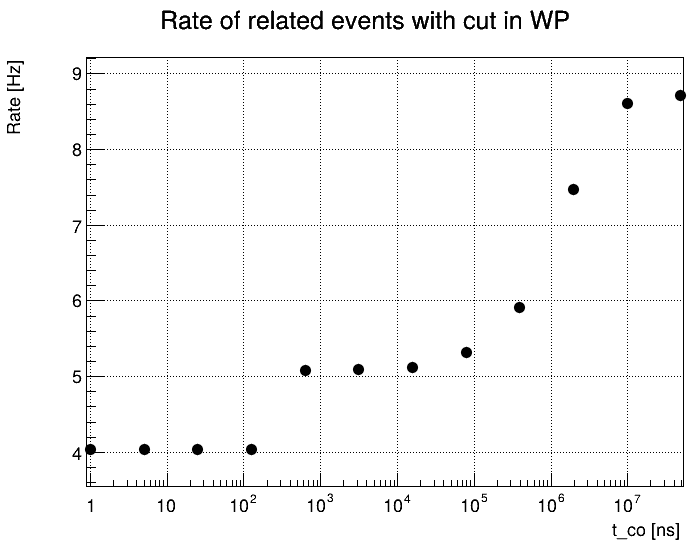
\includegraphics[width=0.49\textwidth]{Risultati/Common_Events_vs_Tolerance_RUN4049_rate_cut_WP_plot.png}
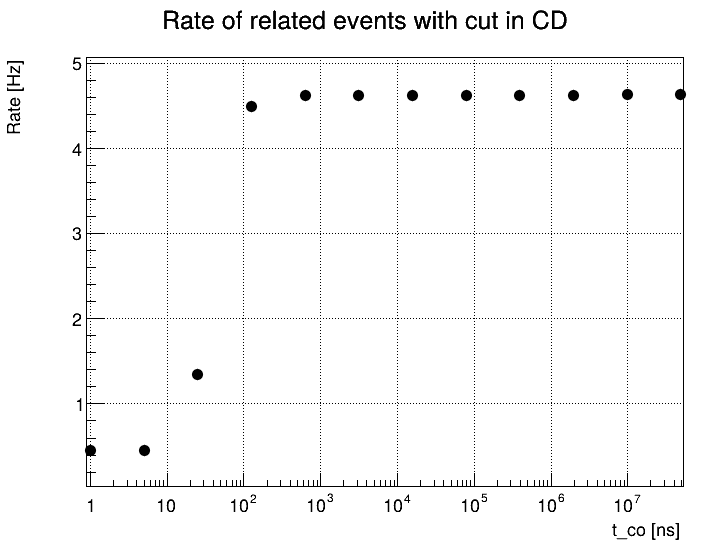
\includegraphics[width=0.49\textwidth]{Risultati/Common_Events_vs_Tolerance_RUN4049_rate_cut_CD_plot.png}

\caption{Rate degli eventi candidati muoni per la RUN4049 in funzione del tempo di tolleranza per il metodo di correlazione temporale. A sinistra è stata applicata la selezione sullo spettro WP, a destra sullo spettro CD.}
\label{Fig:ratez}
\end{figure}
\section{Metodo di clustering di PMT della WP}
\label{sec:wpmuonclassify}
Analogamente a quanto discusso per il primo metodo presentato, un muone che attraversa la Water Pool genera un'elevata quantità di fotoni Cherenkov, poiché deposita una considerevole quantità di energia nel mezzo. Questa intensa emissione luminosa porta all'attivazione di un numero significativo di PMT, causando l'apertura della finestra di trigger. Durante il passaggio di un muone, gruppi di PMT vicini tra loro si attivano (cluster), generando una densità di carica media che varia in funzione della distanza dal centro dell’evento.
\begin{figure}[h!]
\centering
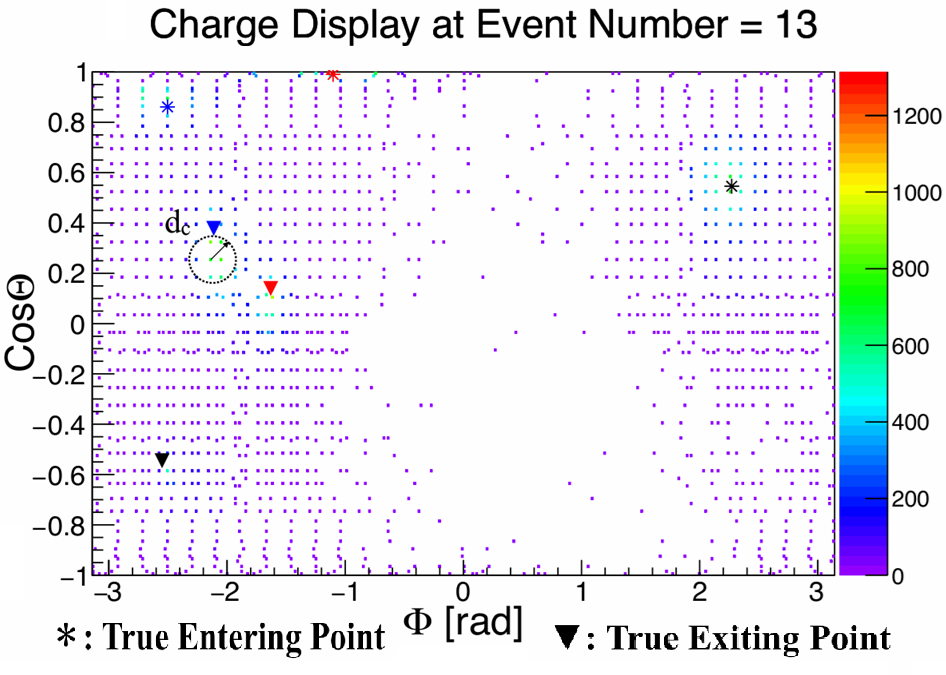
\includegraphics[width=0.6\textwidth]{Immagini/akira1.png}
\caption{Rappresentazione angolare dei PMT della Water Pool attivati, con valore di carica (in fotoelettroni) prodotta indicato dalla scala cromatica. I simboli rappresentano i punti di entrata e uscita simulati dell'evento.}
\label{Fig:akira}
\end{figure}
La Figura \ref{Fig:akira} riporta la carica raccolta dai PMT della WP in scala di colore, con le variabili angolari sferiche $\cos{\Theta}$ e $\Phi$ e ogni punto identifica un PMT. Il metodo di clustering, chiamato WpMuonClassifyRecTool permette di stimare la densità di fotoni prodotti a una certa distanza, come illustrato dalla seguente equazione:
\begin{equation} 
    \rho_\text{Q}=\frac{1}{N_{d<d_c}}\sum_{i(d<d_c)}Q_i 
    \label{eq:photo}
\end{equation}
dove $\rho_\text{Q}$ rappresenta la densità della carica media calcolata, $Q_i$ è la carica osservata nell'i-esimo PMT, e $N_{d < d_c}$ è il numero di PMT attivati nel cluster entro una distanza $d_c$, calibrata in base a simulazioni Monte Carlo.

Una volta ottenuta la carica media, viene determinata la distanza minima tra i PMT con una carica media superiore rispetto agli altri nella WP. Questo consente di individuare la regione in cui è stata raccolta la maggiore quantità di carica. Successivamente, il punto di ingresso del muone viene ricostruito attraverso una media pesata sulla carica raccolta delle posizioni dei PMT del cluster. Utilizzando un metodo simile, che tiene conto della dimensione del cluster e dei punti di ingresso ed uscita, vengono anche classificati gli eventi di muoni bundle. Poiché la ricostruzione è indipendente dal tempo, il metodo identifica come punto di entrata il cluster di PMT situato all'altezza maggiore rispetto al secondo punto. Di conseguenza, gli eventi attesi provenienti dal basso (circa $<1\%$), dovuti all’interazione di neutrini atmosferici, risultano con una traccia ricostruita invertita, ovvero con i punti di ingresso e uscita scambiati.
In sintesi, questo metodo consente di classificare eventi candidati muone e caratterizzare la traccia. Poiché elabora esclusivamente i dati provenienti dalla Water Pool, è in grado di funzionare indipendentemente dallo stato di riempimento del liquido scintillante all'interno del Central Detector.
\subsection{Analisi dati e risultati ottenuti}
Per valutare la stabilità nell'acquisizione dei dati o la presenza di anomalie, ho analizzato l'andamento del rate dei muoni in funzione del tempo di trigger assoluto, in intervalli di $300\,\unit{s}$. Come si può osservare dal grafico \ref{Fig:muon_rate}, non sono presenti anomalie rilevanti e il rate risulta stabile. Questa conclusione è valida, salvo per alcune delle prime \textit{Run} analizzate, che presentano errori di acquisizione o sono state utilizzate per scopi di calibrazione.
\begin{figure}[h!]
\centering
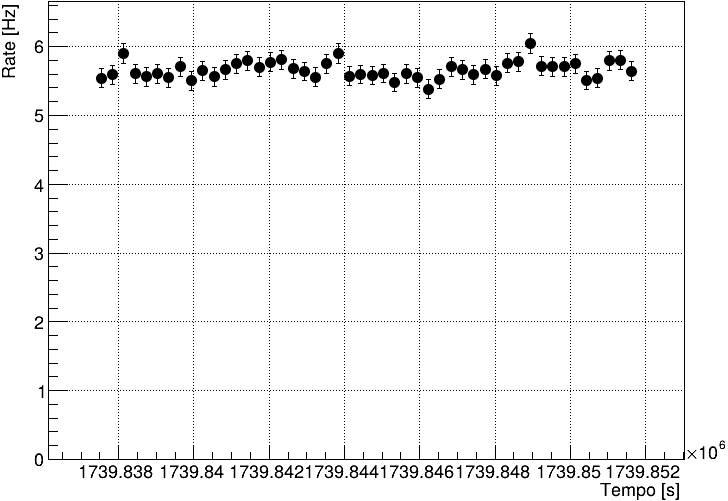
\includegraphics[width=0.6\textwidth]{Risultati/MuonRate_RUN4049mod.png}
\caption{Rate dei muoni in funzione del tempo assoluto per la RUN4049, considerando intervalli di $300\,\unit{s}$. Le barre di errore sono calcolate assumendo una distribuzione di Poisson per gli eventi.}
\label{Fig:muon_rate}
\end{figure}

Il rate totale calcolato è di:
\begin{equation}
    \text{rate}\,(\text{RUN4049})=(5.66\pm0.02)\,\unit{Hz}
    \label{eq:rateM}
\end{equation}
l'errore è stato calcolato assumendo che il numero di eventi segua la distribuzione di Poisson.

Per quanto riguarda gli eventi bundle, questi costituiscono il $18.40\%$ del totale degli eventi registrati per la RUN4049. La distribuzione dei singoli contributi degli eventi bundle è riportata nell'istogramma in Figura \ref{Fig:muon_track}. In linea con le aspettative emerge abbondanza degli eventi singoli e in minor numero eventi bundle con molteplicità maggiore di due.
\begin{figure}[h!]
\centering
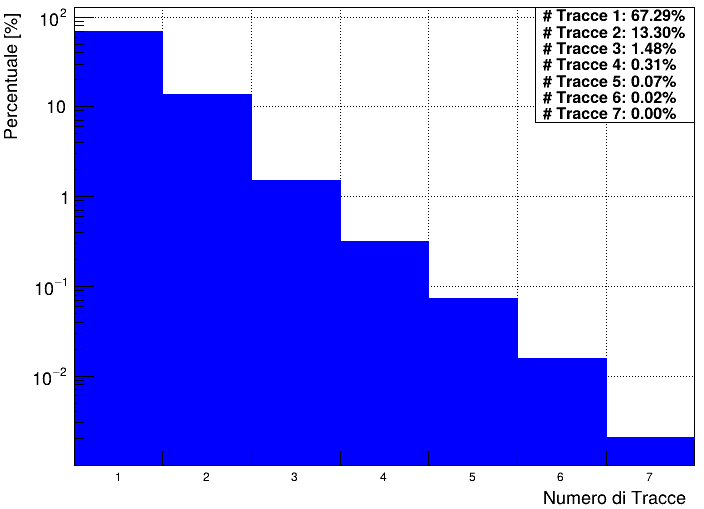
\includegraphics[width=0.55\textwidth]{Risultati/TrackID_Distribution_RUN4049.png}
\caption{Distribuzione percentuale degli eventi muone ricostruiti come bundle, suddivisi tra muoni singoli, doppi, tripli e superiori per la RUN4049.}
\label{Fig:muon_track}
\end{figure}


Dopo aver analizzato la parte di classificazione di questo metodo, è stata studiata la caratterizzazione del tracciato attraverso le informazioni relative alla posizione e alla direzione degli eventi candidati muoni. Nella Figura \ref{Fig:angleplot} sono riportate le distribuzioni angolari della direzione di propagazione degli eventi: a sinistra il coseno dell'angolo polare e a destra l'angolo azimutale.
\begin{figure}[h!]
    \centering
    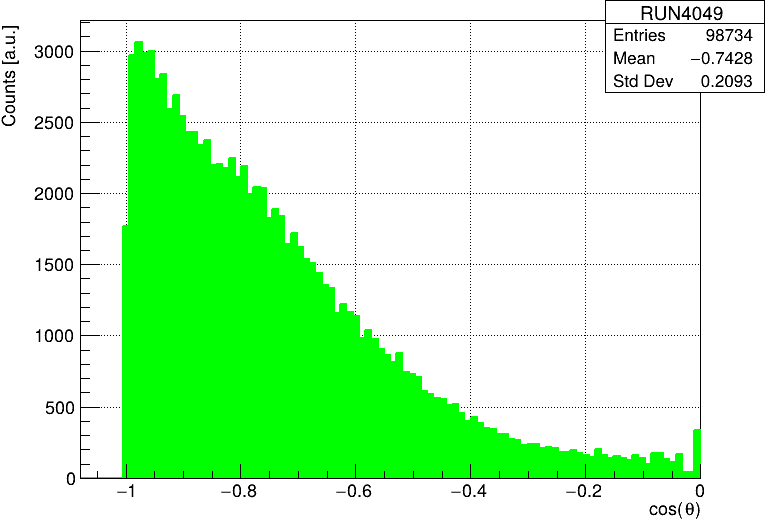
\includegraphics[width=0.495\textwidth]{Risultati/Theta_RUN4049.png}
    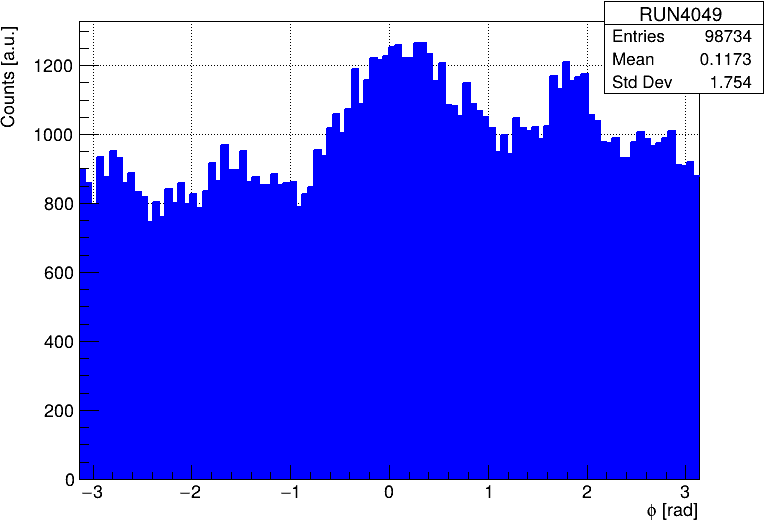
\includegraphics[width=0.495\textwidth]{Risultati/Azimuthal_RUN4049.png}
    \caption{ Per la RUN4049 distribuzione del coseno dell'angolo polare per tutti gli eventi del dataset analizzato, con valori compresi tra $-1$ e $0$ (sinistra). Distribuzione dell'angolo azimutale, con valori compresi tra $-\pi$ e $+\pi$ (destra).}
    \label{Fig:angleplot}
\end{figure}
Come previsto, si osserva una predominanza di eventi con traiettoria quasi verticale discendente. L'analisi dell'angolo azimutale, invece, mostra una distribuzione più complessa da interpretare, influenzata dalla morfologia del territorio circostante. La presenza di montagne, colline o altre formazioni geografiche può infatti schermare in modo differente i muoni cosmici, modificando la distribuzione osservata. Entrambe le distribuzioni mostrano una buona compatibilità con le simulazioni Monte Carlo. Per verificare la presenza di direzioni maggiormente popolate nella propagazione dei muoni, è stata analizzata la correlazione tra l'angolo polare e l'angolo azimutale attraverso un istogramma bidimensionale, riportato in Figura \ref{Fig:polarvsazimuthal}.

\begin{figure}[h!]
\centering
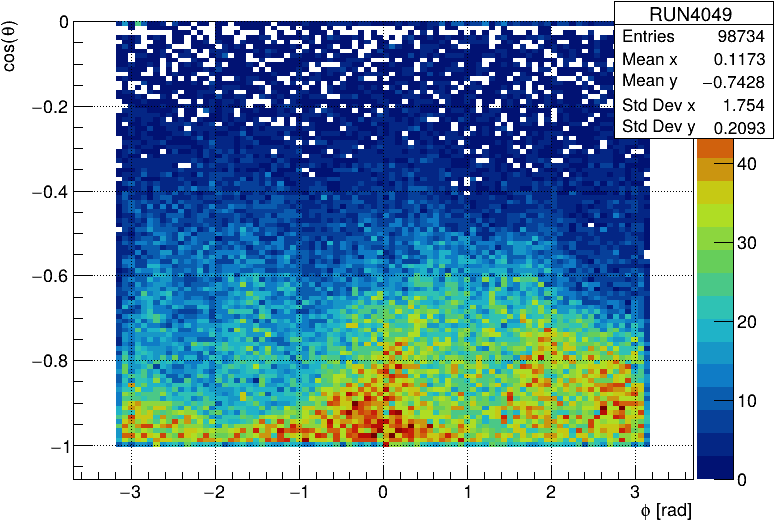
\includegraphics[width=0.7\textwidth]{Risultati/Polar_vs_Azimuthal_Angle_RUN4049.png}
\caption{Correlazione tra il coseno dell'angolo polare $\cos{\theta}$ e l'angolo azimutale $\phi$ degli eventi candidati muoni per la RUN4049 attraverso il metodo di clustering di PMT della WP.}
\label{Fig:polarvsazimuthal}
\end{figure}
Avendo a disposizione i punti di entrata e di uscita, è stato possibile studiare la distanza percorsa dai candidati muoni all'interno del rivelatore. Questo parametro è di fondamentale importanza per la futura implementazione della tecnica di veto, in quanto determinerà la porzione di rivelatore da escludere per ridurre il background prodotto dagli isotopi cosmogenici.
\begin{figure}[h!]
\centering
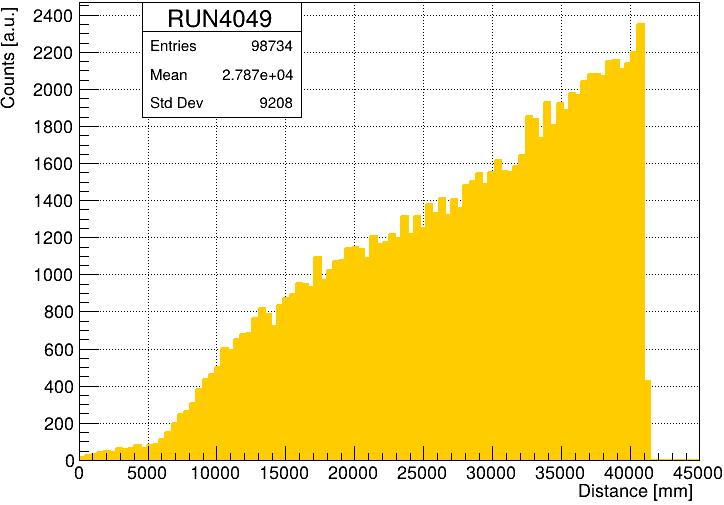
\includegraphics[width=0.6\textwidth]{Risultati/Distance_RUN4049.png}
\caption{Distanza percorsa all'interno del rivelatore per ciascun evento candidato muone registrato nella RUN4049.}
\label{Fig:distance}
\end{figure}
Si osserva che la distanza percorsa può assumere valori superiori al diametro del Central Detector. Calcolando la distanza tra la retta definita dai punti di ingresso e uscita di ciascun evento e l'origine, posizionata al centro del rivelatore, è stato possibile determinare che il $\sim24\%$ degli eventi totali risulta tangente al CD o non lo attraversa direttamente, interagendo invece solo con lo strato d'acqua esterno, ma precedente alla sfera di supporto dei PMT della WP. Questa categoria di muoni è denominata $\mu$-clipping. 

Oltre allo studio delle informazioni legate alla posizione e alla direzione degli eventi candidati muoni ho analizzato la carica depositata. Nella Figura \ref{Fig:charge}, l'istogramma in alto mostra il confronto tra lo spettro di carica dell'intera popolazione di eventi registrati nella Water Pool (in blu) e quello degli eventi classificati come muoni (in rosso). L'istogramma in basso riporta invece la distribuzione degli eventi candidati muone suddivisi in base alla molteplicità dei muoni bundle. 

  %cambaire parole all'interno del grafico e renderlo più grande e leggibile
\begin{figure}[h!]
    \centering
    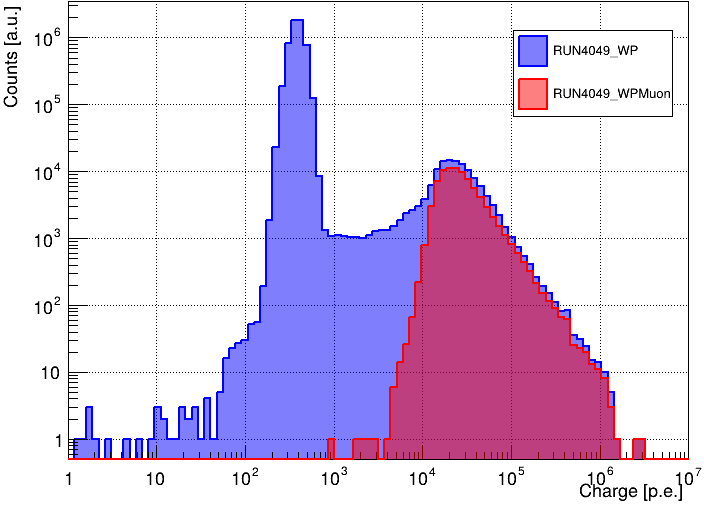
\includegraphics[width=0.57\textwidth]{Risultati/total_PeSum_log_RUN4049.png}
    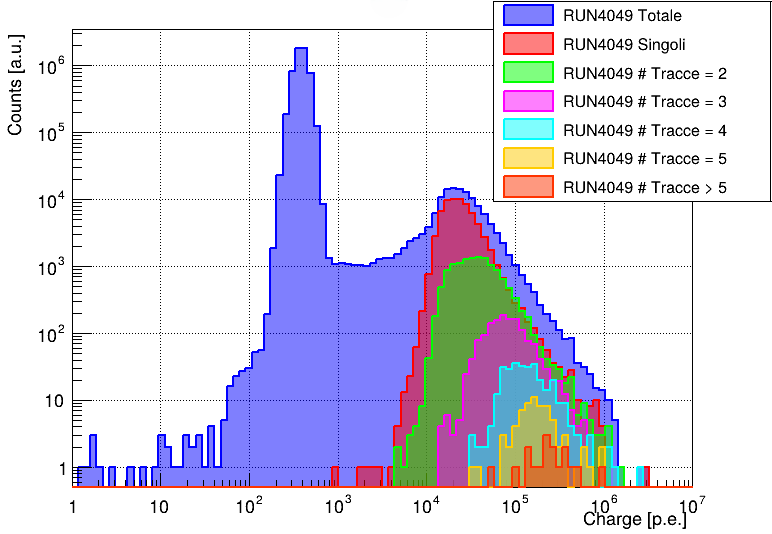
\includegraphics[width=0.67\textwidth]{Risultati/total_PeSum_log_divided_RUN4049.png}
    \caption{Per la RUN4049 spettro della carica totale registrata nella Water Pool sovrapposto allo spettro della carica degli eventi classificati come muoni dal metodo di classificazione mediante clustering di PMT (in alto). Stesso spettro, con gli eventi muone suddivisi in base alla molteplicità degli eventi bundle (in basso).}
    \label{Fig:charge}
\end{figure}
\section{Confronto tra i due metodi di classificazione dei muoni}
I due metodi di classificazione e ricostruzione degli eventi candidati muoni rappresentano un tassello di una più completa strategia per la classificazione dei muoni. Questo lavoro è ancora in fase di ottimizzazione all'interno della collaborazione JUNO, con l'integrazione di ulteriori informazioni e strutture dati, come ad esempio quelle che proverranno dal Top Tracker.

Poiché entrambi i metodi forniscono informazioni sullo spettro della Water Pool, la Figura \ref{Fig:clus} mostra un confronto tra lo spettro della carica ottenuto con il metodo della correlazione temporale (in rosso) e quello derivante dal clustering dei PMT della WP (in verde), sovrapposti allo spettro totale (in blu).

\begin{figure}[h!]
    \centering
    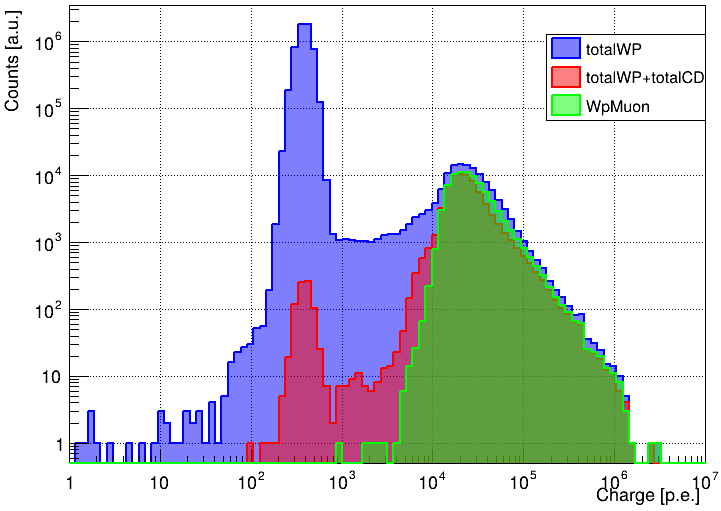
\includegraphics[width=0.7\textwidth]{Risultati/WP_RUN4049_tolerance_200.00m.png}
    \caption{Istogramma degli spettri della carica per la RUN4049. In blu lo spettro della carica degli eventi totali, in rosso lo spettro degli eventi selezionati con il metodo di correlazione temporale e in verde quello ottenuto con il clustering dei PMT. Il tempo di correlazione è fissato a $t_\text{co}=200\,\unit{ns}$}
    \label{Fig:clus}
\end{figure}
L'istogramma, ottenuto fissando $t_\text{co}=200\,\unit{ns}$, evidenzia come quasi la totalità degli eventi identificati dal metodo di correlazione temporale sia inclusa tra quelli selezionati dal metodo di clustering dei PMT. In particolare per eventi ad alta carica (in fotoelettroni), circa il $95\%$ degli eventi candidati muoni dal primo metodo è incluso anche nella selezione effettuata dal secondo. Una prima ragione di questa discrepanza tra i due metodi deriva dal fatto che il metodo basato sul clustering di PMT include tutti i muoni che attraversano la struttura in acciaio inossidabile, mentre il metodo di correlazione temporale seleziona solo gli eventi che attraversano anche il Central Detector. Per quantificare il grado di accordo tra le due metodologie, ho  calcolato l’area di sovrapposizione tra i due spettri, normalizzata rispetto all’area degli eventi identificati dal software WpMuonClassifyRecTool. La Figura \ref{Fig:plis} mostra la dipendenza di questa area di overlap dal tempo di correlazione utilizzato.
\begin{figure}[h!] 
\centering 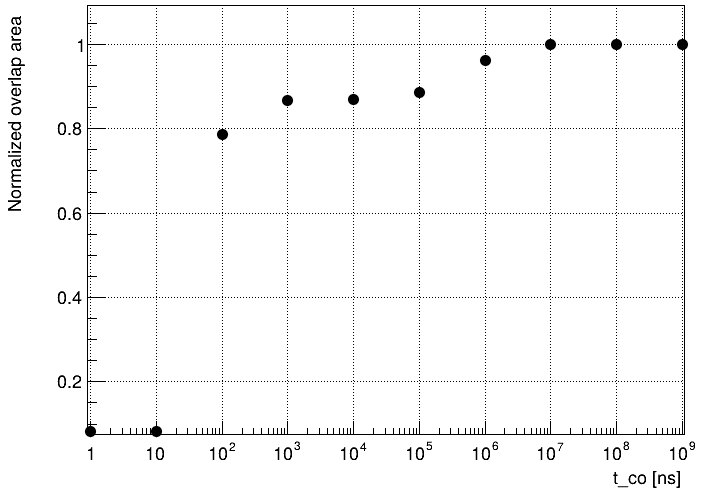
\includegraphics[width=0.5\textwidth]{Risultati/Overlap_Area_vs_Tolerance_RUN4049_plot.png} \caption{Dipendenza dell’area di sovrapposizione tra gli eventi candidati muoni classificati dai due metodi in funzione della finestra temporale di correlazione.} \label{Fig:plis} 
\end{figure}
I valori calcolati per tempi di correlazione molto piccoli e molto grandi confermano la coerenza della scelta di $200\,\unit{ns}$ come valore ragionevole per il confronto. In particolare, tempi eccessivamente ridotti portano a una sovrapposizione nulla, mentre tempi troppo ampi massimizzano la sovrapposizione, includendo però eventi accidentali.


Dai risultati riportati nella tabella \ref{tab:rate_RUN4049} è emerso che, per la RUN4049, i rate calcolati con il metodo di correlazione temporale differiscono da quello ottenuto con il metodo di clustering dei PMT della Water Pool. In particolare, il rate ottenuto applicando il la selezione in carica nello spettro WP è inferiore del $28.6\%$, mentre quello con la selezione in carica nello spettro CD è inferiore del $18.4\%$ rispetto al rate determinato con il secondo metodo. Effettuando lo studio del rate per ogni \textit{Run} analizzata fissando il tempo di correlazione a $200\,\unit{ns}$ ed eseguendo le due diverse selezioni in carica si ottengono i grafici visibili nella Figura \ref{Fig:rateII}. A sinistra è possibile osservare il rate effettuando la selezione in carica nello spettro WP e a destra effettuando la selezione in carica nello spettro CD. Inoltre è possibile osservare nella Figura \ref{Fig:runmuonrate} il rate in funzione degli indici delle \textit{Run} utilizzando il metodo WpMuonClassifyRecTool.
\begin{table}[h!]
    \centering
    \renewcommand{\arraystretch}{1.2}
    \begin{tabular}{|c|c|}
        \hline
        \textbf{Metodo} & \textbf{Rate (RUN4049) [Hz]} \\
        \hline
        Correlazione, selezione in carica WP & $(4.04 \pm 0.02)$ \\
        Correlazione, selezione in carica CD & $(4.62 \pm 0.02)$ \\
        \hline
        Clustering PMT & $(5.66 \pm 0.02)$ \\
        \hline
    \end{tabular}
    \caption{Valori del rate per la RUN4049 ottenuti con i due metodi. L'errore è stato calcolato assumento che il numero di evnti seguano la distribuzione di Poisson.}
    \label{tab:rate_RUN4049}
\end{table}
\begin{figure}[h!]
    \centering
    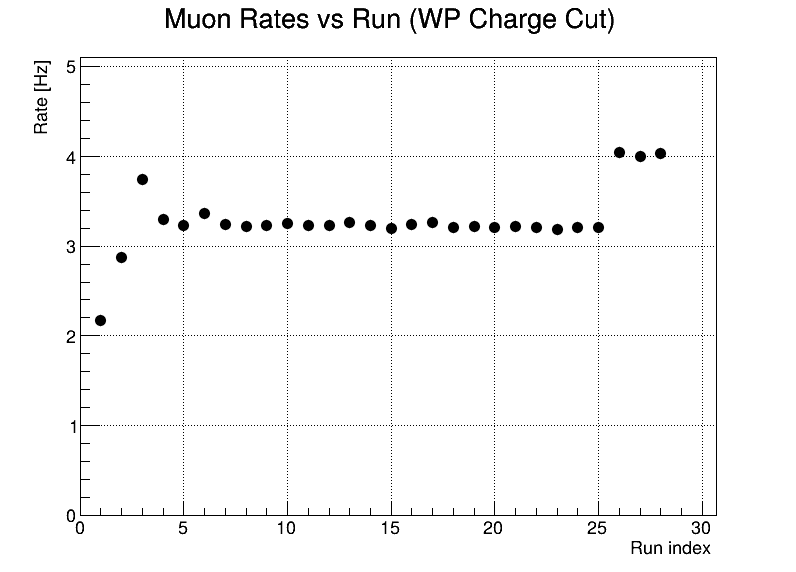
\includegraphics[width=0.49\textwidth]{Risultati/Muon_Rate_vs_Run_with_Energy_Cut_WP.png}
    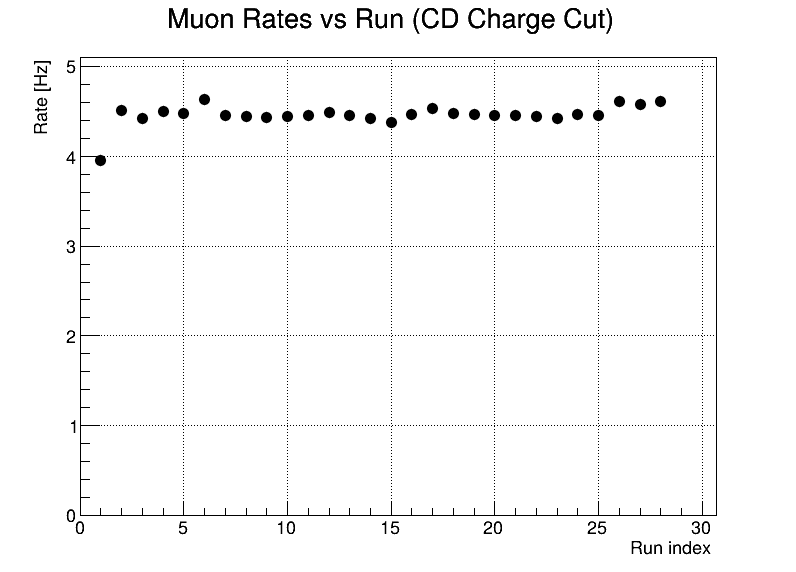
\includegraphics[width=0.49\textwidth]{Risultati/Muon_Rate_vs_Run_with_Energy_Cut_CD.png}
    \caption{Rate in funzione dell'indice della \textit{Run} ordinate cronologicamente utilizzando il metodo di correlazione temporale. A sinistra effettuando la selezione in carica nello spettro WP mentre a destra nello spettro CD. Il tempo di correlazione è fissato a $t_\text{co}=200\,\unit{ns}$.}
    \label{Fig:rateII}
\end{figure}
\begin{figure}[h!]
\centering
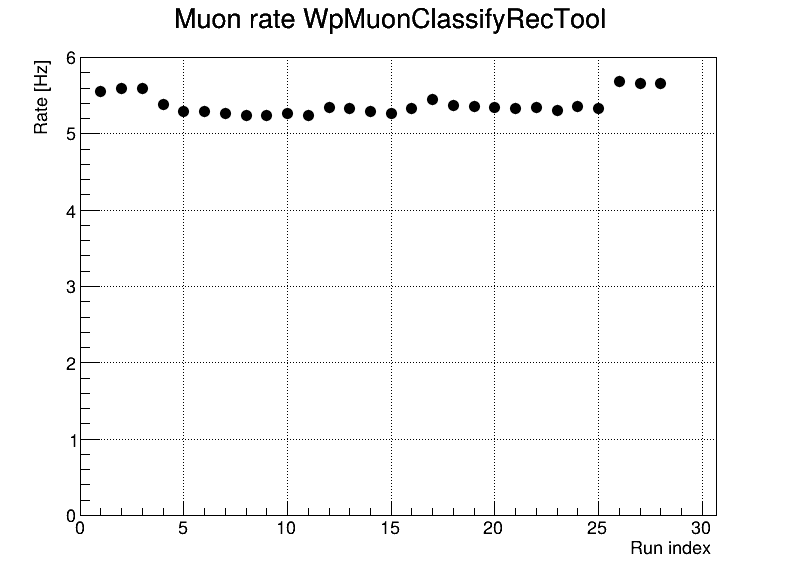
\includegraphics[width=0.6\textwidth]{Risultati/Muon_Rate_vs_Run_EventID_univ.png}
\caption{Andamento del rate dei muoni in funzione dell'indice della \textit{Run} considerata (in ordine cronologico) utilizzando il metodo di classificazione di clustering di PMT. Le barre di errore sono presenti, ma non visibili.}
\label{Fig:runmuonrate}
\end{figure}
\section{Conclusioni}
Nel presente lavoro di tesi sono stati analizzati i dati acquisiti dal rivelatore JUNO nel periodo compreso tra gennaio 2025 e marzo 2025, in una fase tra la fine del riempimento con l'acqua e i primi progressi con il riempimento con LS nel CD. Questo ha permesso di utilizzare JUNO come un vero e proprio rivelatore Cherenkov rendendo possibile uno studio approfondito dei muoni cosmici, attraverso l’implementazione e l’analisi di due metodi di classificazione.

Il primo metodo, sviluppato in questo studio, si basa sulla correlazione temporale tra l’apertura della finestra di trigger dei PMT nella Water Pool e nel Central Detector. Per identificare gli eventi candidati muoni, è stato imposto un tempo di correlazione pari a $200\,\unit{ns}$, valore scelto considerando:
\begin{itemize}
    \item Il tempo di attraversamento del muone (trattato in regime relativistico) lungo il diametro del CD;
    \item Il tempo di propagazione dei fotoni verso i PMT e la successiva generazione del segnale.
\end{itemize}
Tuttavia, questo metodo introduce inevitabilmente una certa frazione di eventi correlati temporalmente in modo casuale, prevalentemente dovuti a rumore di fondo con bassa carica in fotoelettroni. Quindi, sono state definite due soglie di carica in fotoelettroni, derivate dall’analisi degli spettri della Water Pool e del Central Detector: $E^\text{WP}_\text{th} = 5\cdot10^3\,\text{p.e.}$ e $E^\text{CD}_\text{th} = 5\cdot10^4\,\text{p.e.}$. L’applicazione di questi criteri ha permesso di ottenere una misura del rate degli eventi candidati muoni per ogni \textit{Run}, con i risultati riportati nella Figura \ref{Fig:rateII}. Tuttavia, questo metodo non fornisce informazioni sulla posizione o sulla direzione delle tracce dei singoli eventi.

Il secondo metodo, invece, è integrato nel software ufficiale di JUNO e si basa su un approccio di clustering dei PMT. Identificando gruppi di fotomoltiplicatori attivati, è in grado di classificare gli eventi candidati muoni e fornire informazioni dettagliate come la posizione del centro del cluster, il numero di tracce presenti all'interno di ciascun evento e la carica totale in fotoelettroni associata. A differenza del primo metodo, questo metodo non utilizza alcuna informazione temporale e analizza solo i dati provenienti dalla Water Pool. Sono state condotte diverse analisi sulle grandezze ricostruite e il rate degli eventi candidati muoni ottenuto con questo approccio è riportato nella Figura \ref{Fig:runmuonrate}.

Entrambi i metodi hanno prodotto risultati coerenti e plausibili, offrendo due approcci indipendenti per classificare eventi candidati muoni. Questi studi rappresentano solo una piccola parte del lavoro verso l’ottimizzazione della strategia di identificazione e classificazione dei muoni in JUNO. Il lavoro è ancora in corso, con l'obiettivo di integrare ulteriori informazioni e strutture, come il Top Tracker, per una caratterizzazione ancora più precisa dei muoni cosmici nel rivelatore.
